\documentclass{myreport}

\begin{document}

\maketitle

% 目录
\newpage
\tableofcontents
\newpage

% 正文
\section{系统需求分析}
  \subsection{需求概述}
    \subsubsection{课程设计要求}
      对于排课管理系统, 课程设计的要求如下:
      \begin{itemize}
        \item 实现班级, 课程等基本信息的管理;
        \item 实现学生, 教师信息的管理;
        \item 实现班级课程及课程的任课教师和排课管理;
        \item 创建存储过程检测指定教师, 指定节次是否有课;
        \item 创建存储过程生成指定班级的课程表;
        \item 创建存储过程生成指定老师的课程表;
        \item 建立数据库相关表之间的参照完整性约束.
      \end{itemize}
    \subsubsection{实体集}
      即通过数据库自动排课并提供给学生查询,让学生和老师可以查询具体时间安排.
      该系统可以通过以下实体集实现
      \begin{itemize}
        \item \emph{教学楼}实体集, 包含楼号和楼名;
        \item \emph{教室}实体集, 包含楼号,教室号和容量;
        \item \emph{院系}实体集, 包含院系编号和院系名;
        \item \emph{课程}实体集, 包含课程号, 课程名, 课程类型, 开课学院;
        \item \emph{教师}实体集, 包含教师的编号, 姓名,院系, 职称, 研究方向\footnote{可能是老师工作的具体院系, 如"计算机系", 也可能是其他研究所,如"基础数学研究所"};
        \item \emph{班级}实体集, 班级ID, 班级名, 人数, 所属院系;
      \end{itemize}

  \subsection{组织结构分析}
    本系统适用于教师与学生对课程的管理, 提供给学生,教师所有表的查看权限, 数据库管理员拥有其他权限.

  \subsection{管理功能分析}
    排课是个综合系统,需要从教务系统中导入数据(或者由数据库管理员人工导入),实现课程安排,即课程管理, 同时将课程的信息分别存储汇总, 部分实现教师管理, 时间管理,教室管理, 班级管理(如    \cref{fig:function}
    ).
    \begin{figure}[H]
      \centering
      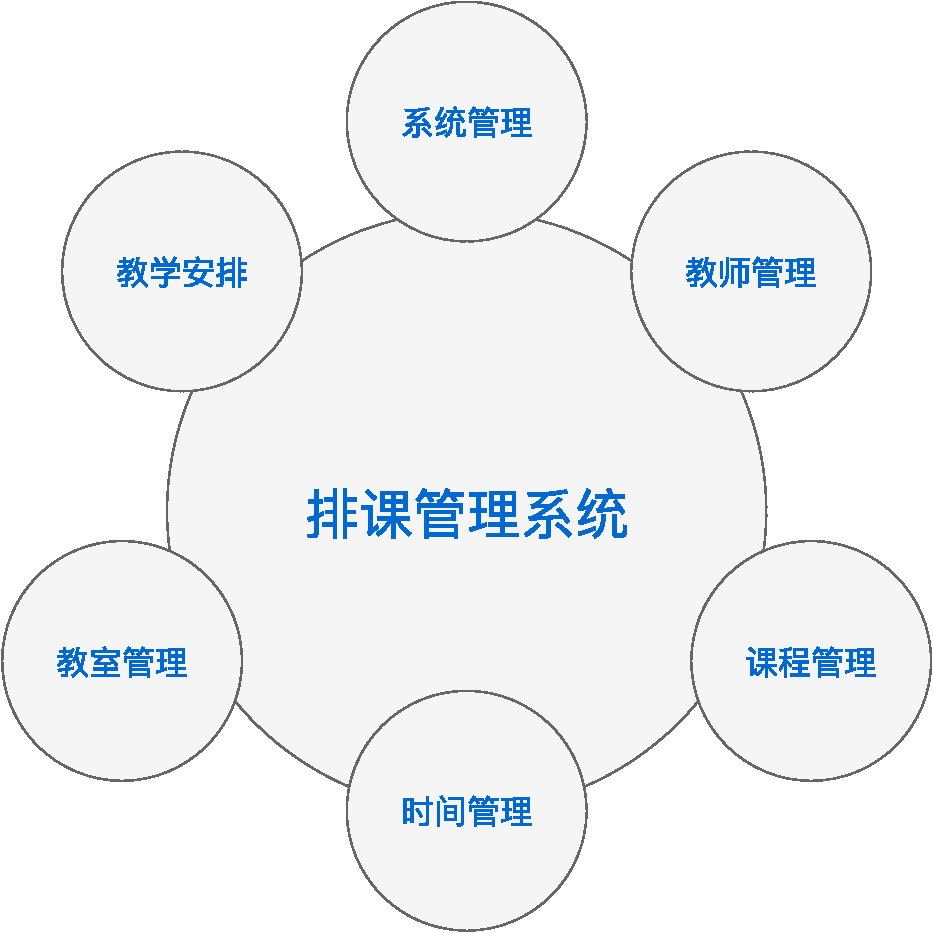
\includegraphics[width = 0.6\textwidth]{function}
      \caption{排课系统的管理功能}
      \label{fig:function}
    \end{figure}

  \subsection{业务流分析}
    \subsubsection{管理员业务}
      管理员业务如图\cref{fig:manager_function}
      \begin{figure}[H]
        \centering
        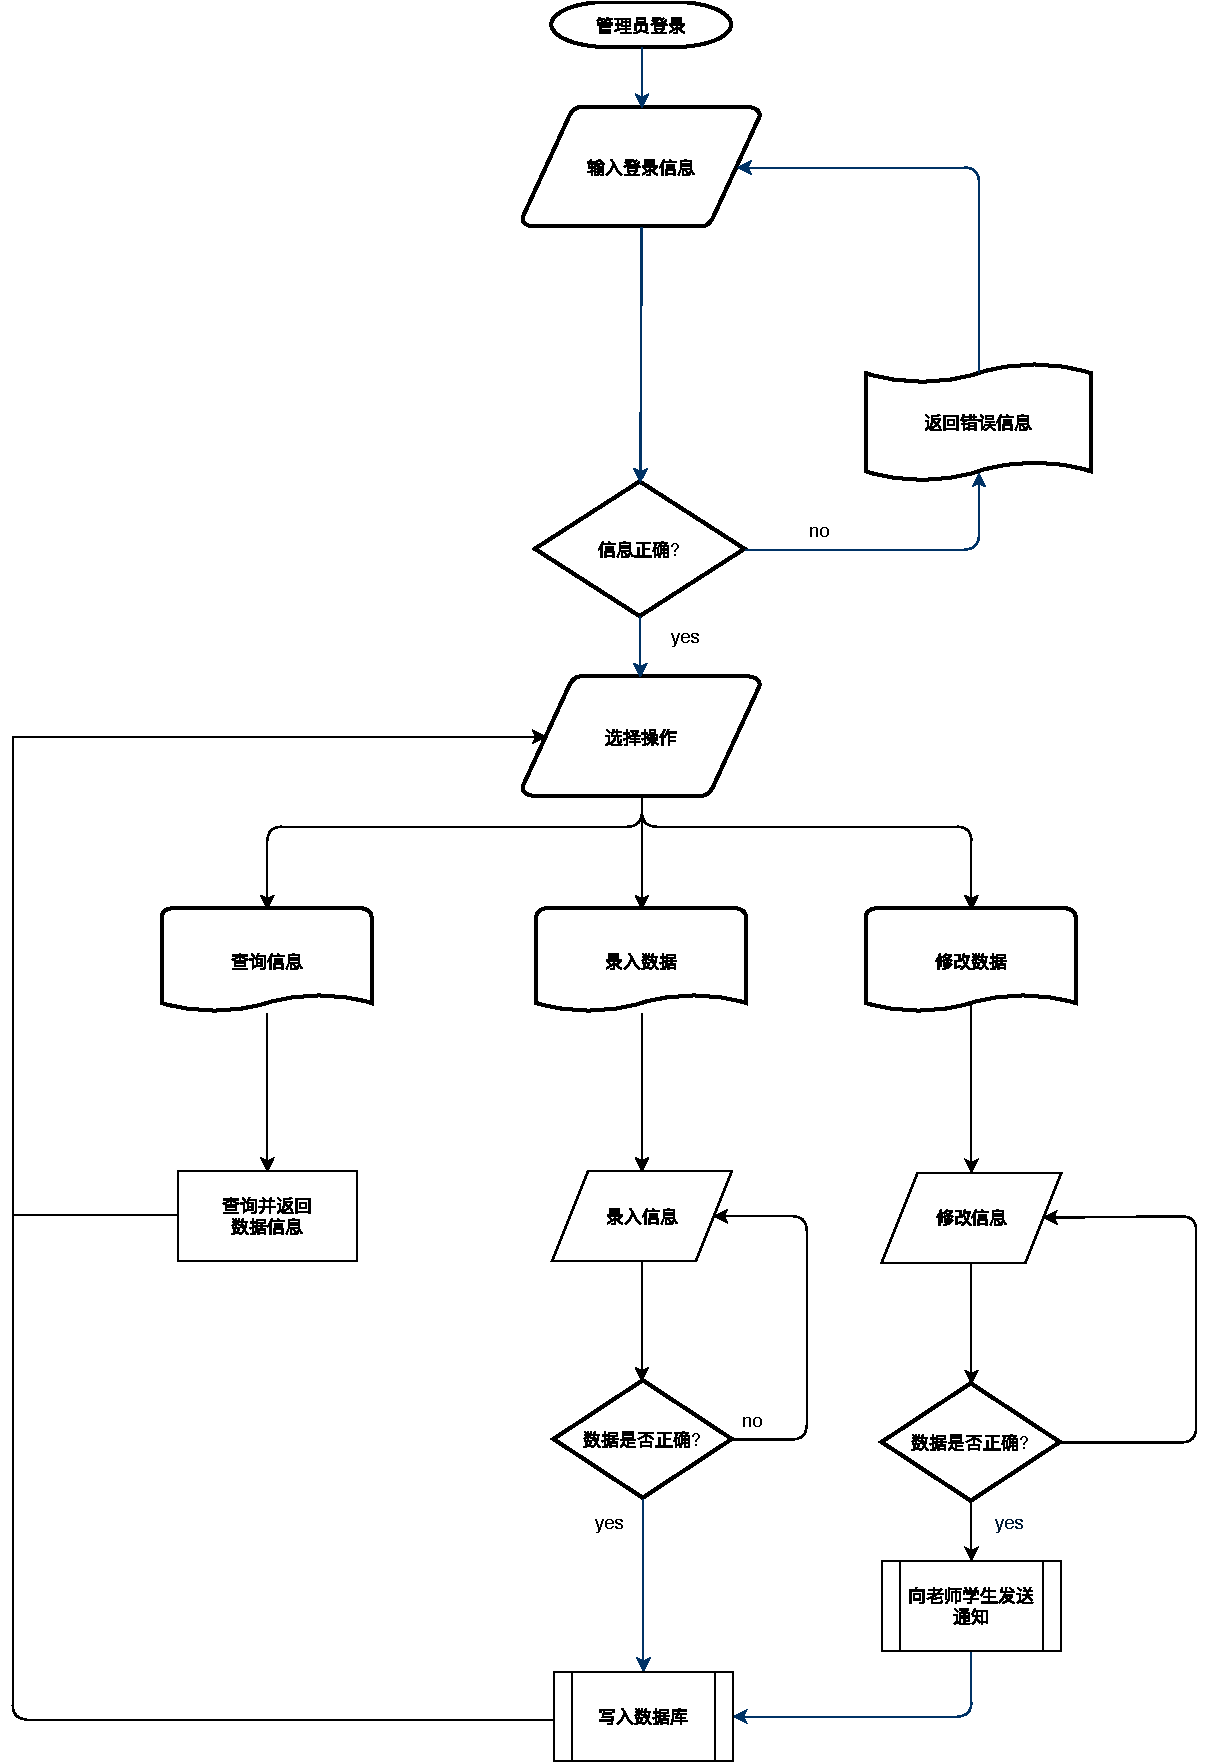
\includegraphics[width = \textwidth]{manager_function}
        \caption{管理员的业务流}
        \label{fig:manager_function}
      \end{figure}
    \subsubsection{教师查询}
      教师的业务如
      \cref{fig:teacher_function}
      \begin{figure}[H]
        \centering
        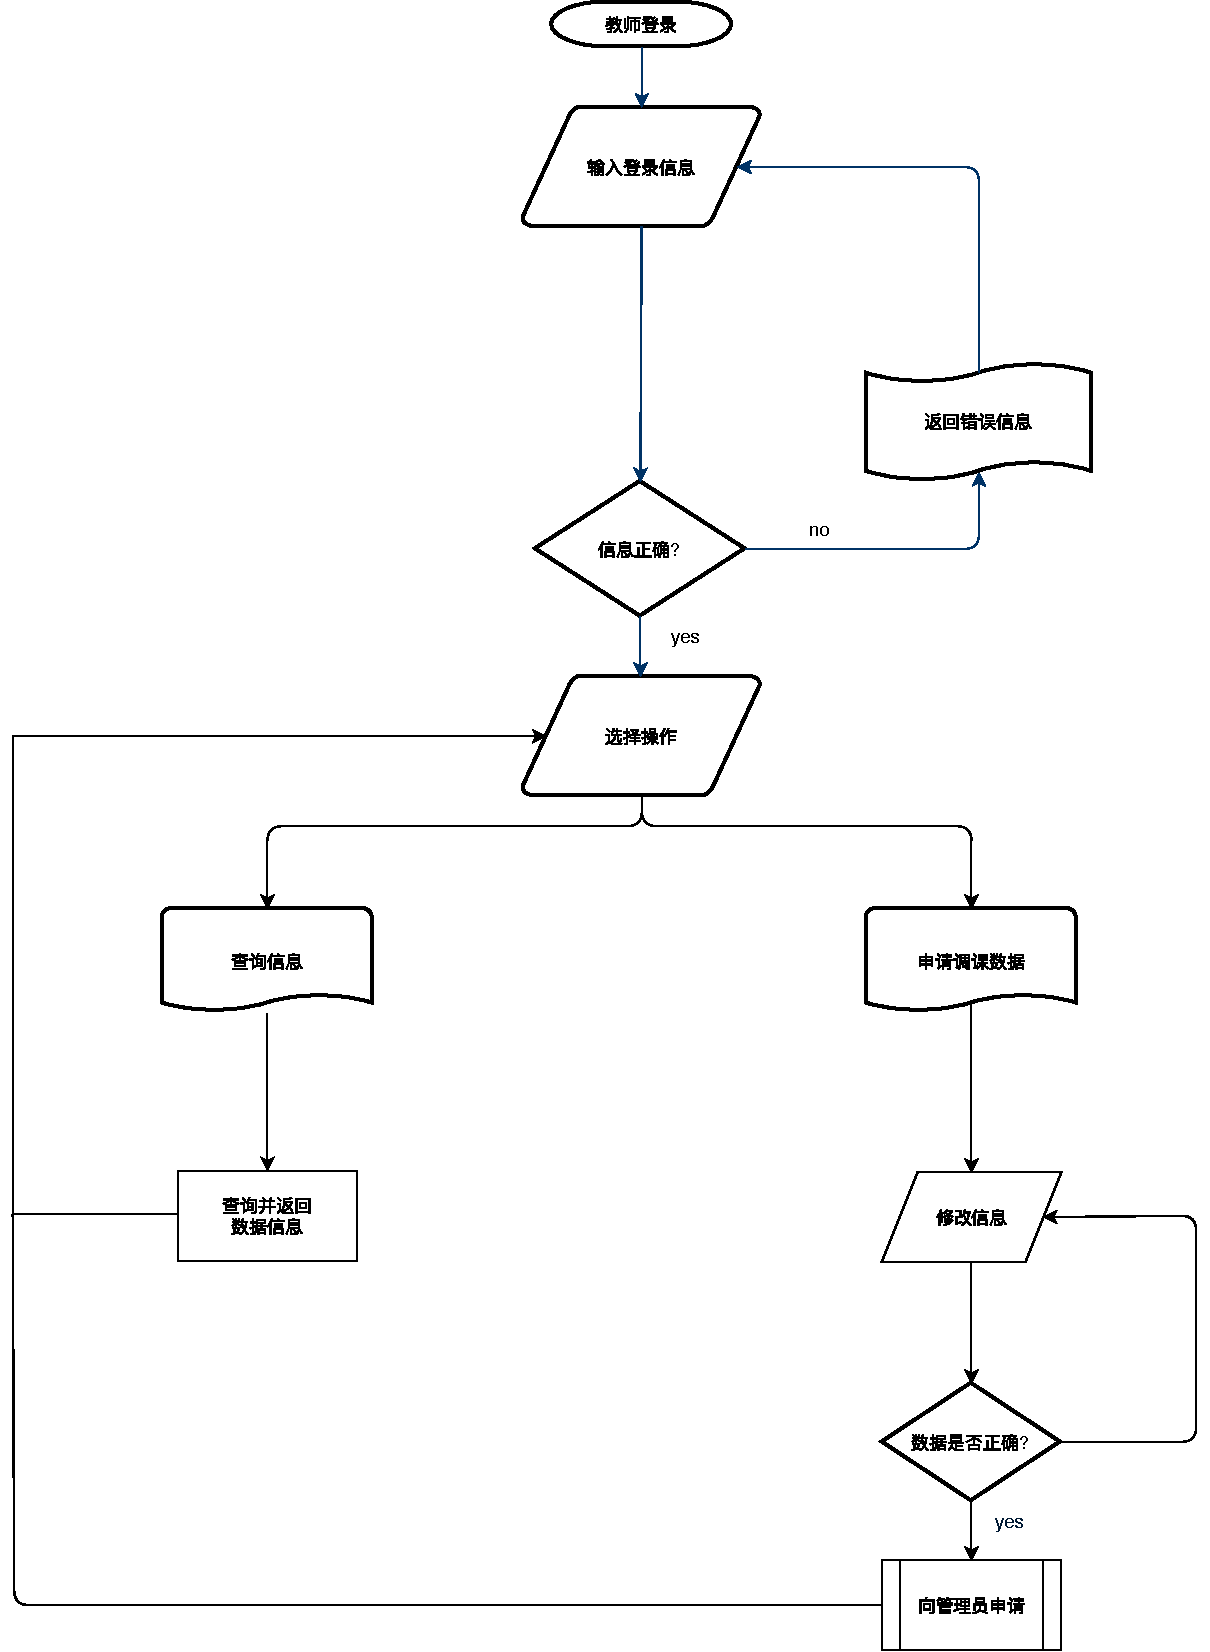
\includegraphics[width = 0.8\textwidth]{teacher_function}
        \caption{教师业务流程}
        \label{fig:teacher_function}
      \end{figure}

  \subsection{数据流分析}
    系统外部环境图如
    \cref{fig:outer}
    \begin{figure}[H]
      \centering
      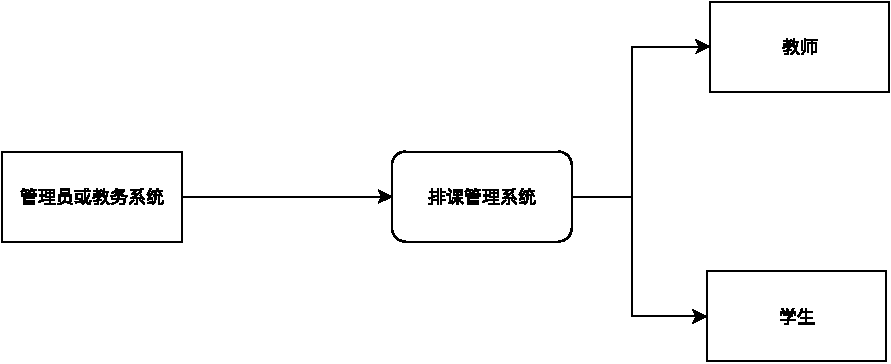
\includegraphics[width = 0.6\textwidth]{outer}
      \caption{系统外部环境图}
      \label{fig:outer}
    \end{figure}

    接下来将模型细化,
    \cref{fig:dataflow_1}
    描绘了系统的主要功能
    \begin{figure}[H]
      \centering
      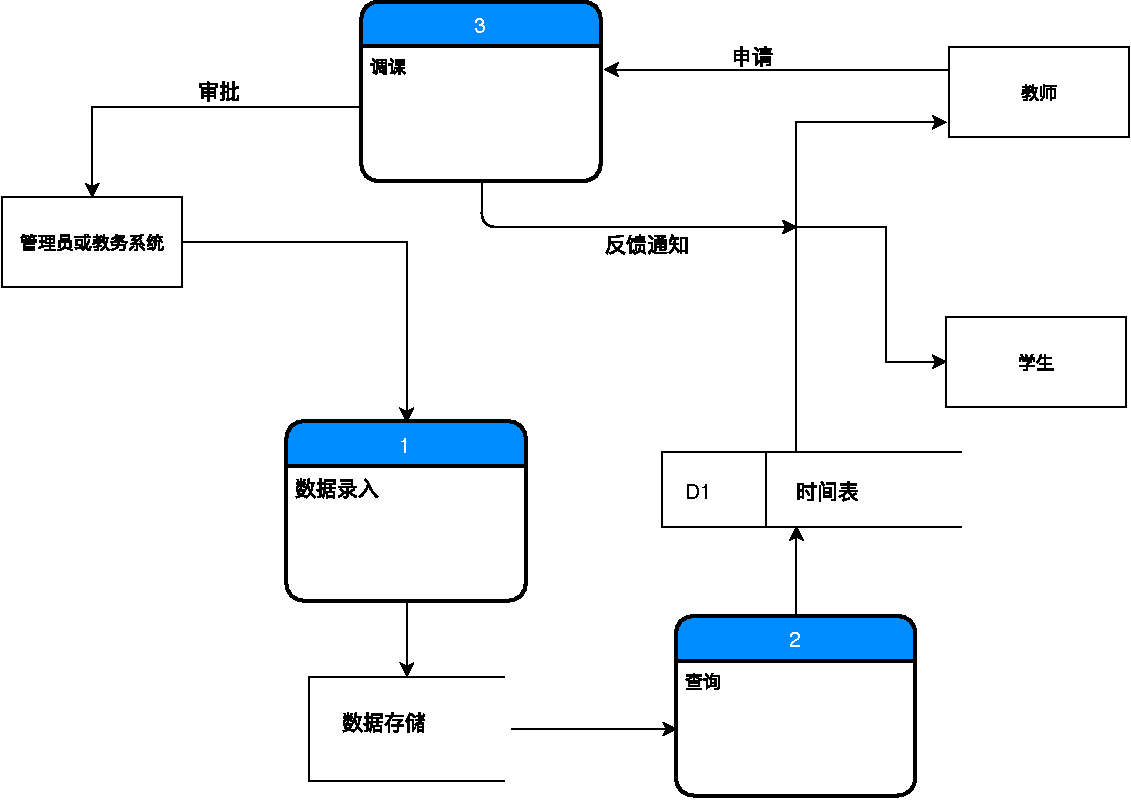
\includegraphics[width = \textwidth]{dataflow_1}
      \caption{排课系统功能的第一层数据流图}
      \label{fig:dataflow_1}
    \end{figure}

  \subsection{数据字典}
    \subsubsection{数据字典}

      根据数据流图中所涉及的信息,并对信息进行相应的分析,确定出所有数据项的描述内容,其主要分为数据项名称、类型、长度和取值范围,如\cref{t:data_dict}所示

      \begin{longtabu} to \textwidth {clcXXX}
        \caption{数据字典(具体的数据的大小参考\cite{tinyint})}
        \label{t:data_dict} \\
        \toprule[1.5pt]
          \makebox[0.1\textwidth]{名称}  &
          \makebox[0.2\textwidth]{含义} &
          \makebox[0.1\textwidth]{类型} &
          \makebox[0.1\textwidth]{大小} &
          \makebox[0.1\textwidth]{取值范围} &
          \makebox[0.2\textwidth]{备注} \\
        \midrule[1pt]
        \endhead

        \bottomrule[1.5pt]
        \endfoot


        % 表格正文
          楼号    & 教学楼的编号 & tinyint & \SI{1}{B} & 0-255 & \\
          楼名    & 教学楼的名称 & char(5) & \SI{15}{B} & 长度$\le 5$ & \\
          容量    & 教学楼的容量 & tinyint & \SI{1}{B} & 0-255 & \\
          院系编号 & 院系的编号 & tinyint & \SI{1}{B} & 0-255 & \\
          院系名   & 院系名 & char(8) & $\le\SI{24}{B}$ & 0-255 & \\
          课程号   & 课程编号 & char(20) & \SI{20}{B} & 20位 & \\
          课程名   & 课程名 & char(10) & $\le \SI{30}{B}$ & 10位 & \\
          类型名   & 课程的类型 & char(10) & $\le \SI{30}{B}$ & \\
          教师号   & 教师编号 & char(20) & \SI{20}{B} & 20位 & \\
          教师名   & 教师的姓名 & char(10) & $\le \SI{30}{B}$ & \\
          职称     & 教师的职称 & char(3) &\SI{9}{B}  & 助教, 讲师, 副教授, 教授 \\
          班号     & 班级编号 & char(20) & \SI{20}{B} & 20位 & \\
          班名     & 班级的全名 & char(10) & $\le \SI{30}{B}$ & \\
          人数     & 班级人数 & tinyint & \SI{1}{B} & 0-255 & \\
          时间号   & 上课时间的标识 & char(20) & \SI{20}{B} & 20位 & \\
          日       & 星期几 & tinyint & \SI{1}{B} & 0-255 & 星期用1-5代替\\
          开始时间 & 上课时间 & tinyint & \SI{1}{B} & 0-255 & 假设上课时间都是整点, 24小时制\\
          结束时间 & 下课时间 & tinyint & \SI{1}{B} & 0-255 & 假设下课时间都是整点, 24小时制\\
          开始周   & 第几周开始 & tinyint & \SI{1}{B} & 0-255 & \\
          结束周   & 第几周结束 & tinyint & \SI{1}{B} & 0-255 & \\
          is\_odd  & 单周上课 & bit & \SI{1}{B} & 0,1 & 默认为1 \\
          is\_even & 双周上课 & bit & \SI{1}{B} & 0,1 & 默认为1 \\
          节号      & 上课节的标识 & char(20) & \SI{20}{B} & 20位 & \\
          学期      & 在上学期或下学期 & bit & \SI{1}{B} & 0,1 & 每年第一学期为0,第二学期为1 \\
          年        & 年份 & smallint & \SI{2}{B} &$-32,768$- $32,767$ & \\

          % \specialrule{0em{8pt}{1pt}}
      \end{longtabu}
    \subsubsection{数据结构}

      根据数据流图中的信息的分析,在数据项描述的基础上确定所有数据结构的描述,
      主要有数据结构名称、含义和组成说明。
      本题数据结构如\cref{t:data_structure}.

      \begin{table}[H]
        \caption{数据结构说明}
        \label{t:data_structure}
        \centering
        \begin{tabularx}{\textwidth}{ccX}
        \toprule[1.5pt]
          \makebox[0.1\textwidth]{名称} &
          \makebox[0.4\textwidth]{含义} &
          \makebox[0.5\textwidth]{组成}  \\
          \midrule[1pt]
          $build$ & 教学楼信息 & 楼号, 楼名 \\
          $classroom$ & 教室信息 & 楼号, 教室号, 容量 \\
          $department$ & 院系 & 院系号, 院系名 \\
          $course$ & 课程信息 & 课程号, 课程名, 课程类型, 开课院系编号 \\
          $instructor$ & 老师信息 & 编号, 姓名, 职称, 院系编号, 研究方向 \\
          $class$ & 班级 & 班号, 班级名, 人数, 院系号 \\
          $time\_slot$ & 上课时间信息 & 时间标识符, 上课日, 上课时间, 下课时间, 开始周, 结束周, 单周上课, 双周上课 \\
          $section$ & 每节课的信息 & 课程编码,时间标识, 课程号, 学期, 开课年, 楼号, 教室号. \\



          % \specialrule{0em{8pt}{1pt}}
        \bottomrule[1.5pt]
        \end{tabularx}
      \end{table}

    \subsubsection{数据流描述}
      根据数据流图的数据流向的分析,确定所有数据流的描述,如
      \cref{t:dataflow}

      \begin{table}[H]
        \caption{数据流描述}
        \label{t:dataflow}
        \centering
        \begin{tabular}{cccc}
        \toprule[1.5pt]
          \makebox[0.2\textwidth]{数据流名} &
          \makebox[0.3\textwidth]{数据流来源} &
          \makebox[0.2\textwidth]{数据流去向} &
          \makebox[0.3\textwidth]{说明}
          \\
          \midrule[1pt]
          课程信息 & 管理员导入 & 学生,教师查询 & 记录每门课的信息 \\
          教师信息 & 管理员导入 & 学生,教师查询 & 记录教师的信息 \\
          教室信息 & 管理员导入 & 学生,教师查询 & 记录教室的信息 \\
          教学楼信息 & 管理员导入 & 学生,教师查询 & 记录教学楼的信息 \\
          调课申请 & 教师申请 & 管理员处理 & 调整上课信息 \\
          调课通知 & 管理员处理 & 学生,教师通知 & 调整上课信息 \\
          关注课程 & 学生,教师设置 & 用户自己查询 & 学生教师关注上课信息 \\
          个人课表 & 数据库 & 用户查询 & 可以设置显示关注课程 \\
          % \specialrule{0em{8pt}{1pt}}
        \bottomrule[1.5pt]
        \end{tabular}
      \end{table}


\section{数据库概念结构设计}
  \subsection{实体分析}
    经需求分析,本系统中包含六个实体,包含
    教学楼,教室,院系,课程,教师,班级
  \subsection{属性分析}
    \begin{itemize}
      \item \emph{教学楼}实体集, 包含楼号和楼名;
      \item \emph{教室}实体集, 包含楼号,教室号和容量;
      \item \emph{院系}实体集, 包含院系编号和院系名;
      \item \emph{课程}实体集, 包含课程号, 课程名, 课程类型, 开课学院;
      \item \emph{教师}实体集, 包含教师的编号, 姓名,院系, 职称, 研究方向\footnote{可能是老师工作的具体院系, 如"计算机系", 也可能是其他研究所,如"基础数学研究所"};
      \item \emph{班级}实体集, 班级ID, 班级名, 人数, 所属院系;
    \end{itemize}
  \subsection{联系分析}

      % 用户与图书有查看和购买联系,用户可以查看并购买图书,同时用户购买图书即生成一个订单,是用户和订单的联系;每个用户生成的不同订单集合到订单列表,两者之间有详细信息的联系;管理员与图书和图书分类有管理联系,管理员通过进货入库和销售出库对于图书详细信息进行更改;同时管理员可以查看订
      % 单,对其有管理权限。
    \begin{itemize}
      \item 教室对教学楼有位置联系, 即教室位于特定教学楼;
      \item 教室,课程与时间存在联系, 每个课程在特定时间的特定教室上课;
      \item 课程老师存在联系, 某个课程由特定老师负责;
      \item 班级与学院存在联系, 一个班级属于一个学院;
      \item 老师与院系存在联系, 老师属于院系;
    \end{itemize}


  \subsection{概念模型设计}
    经过需求分析和实体属性分析,
    以及各实体之间的关系分析,
    最终得到概念模型如
    \cref{fig:concept_model}\footnote{访问\url{https://app.sqldbm.com/SQLServer/Share/3gOZcBDE7lI7tlvWVLWffUGFrngIE8md_DYjF4jNYw0}可在线查看}
    \begin{figure}[H]
      \centering
      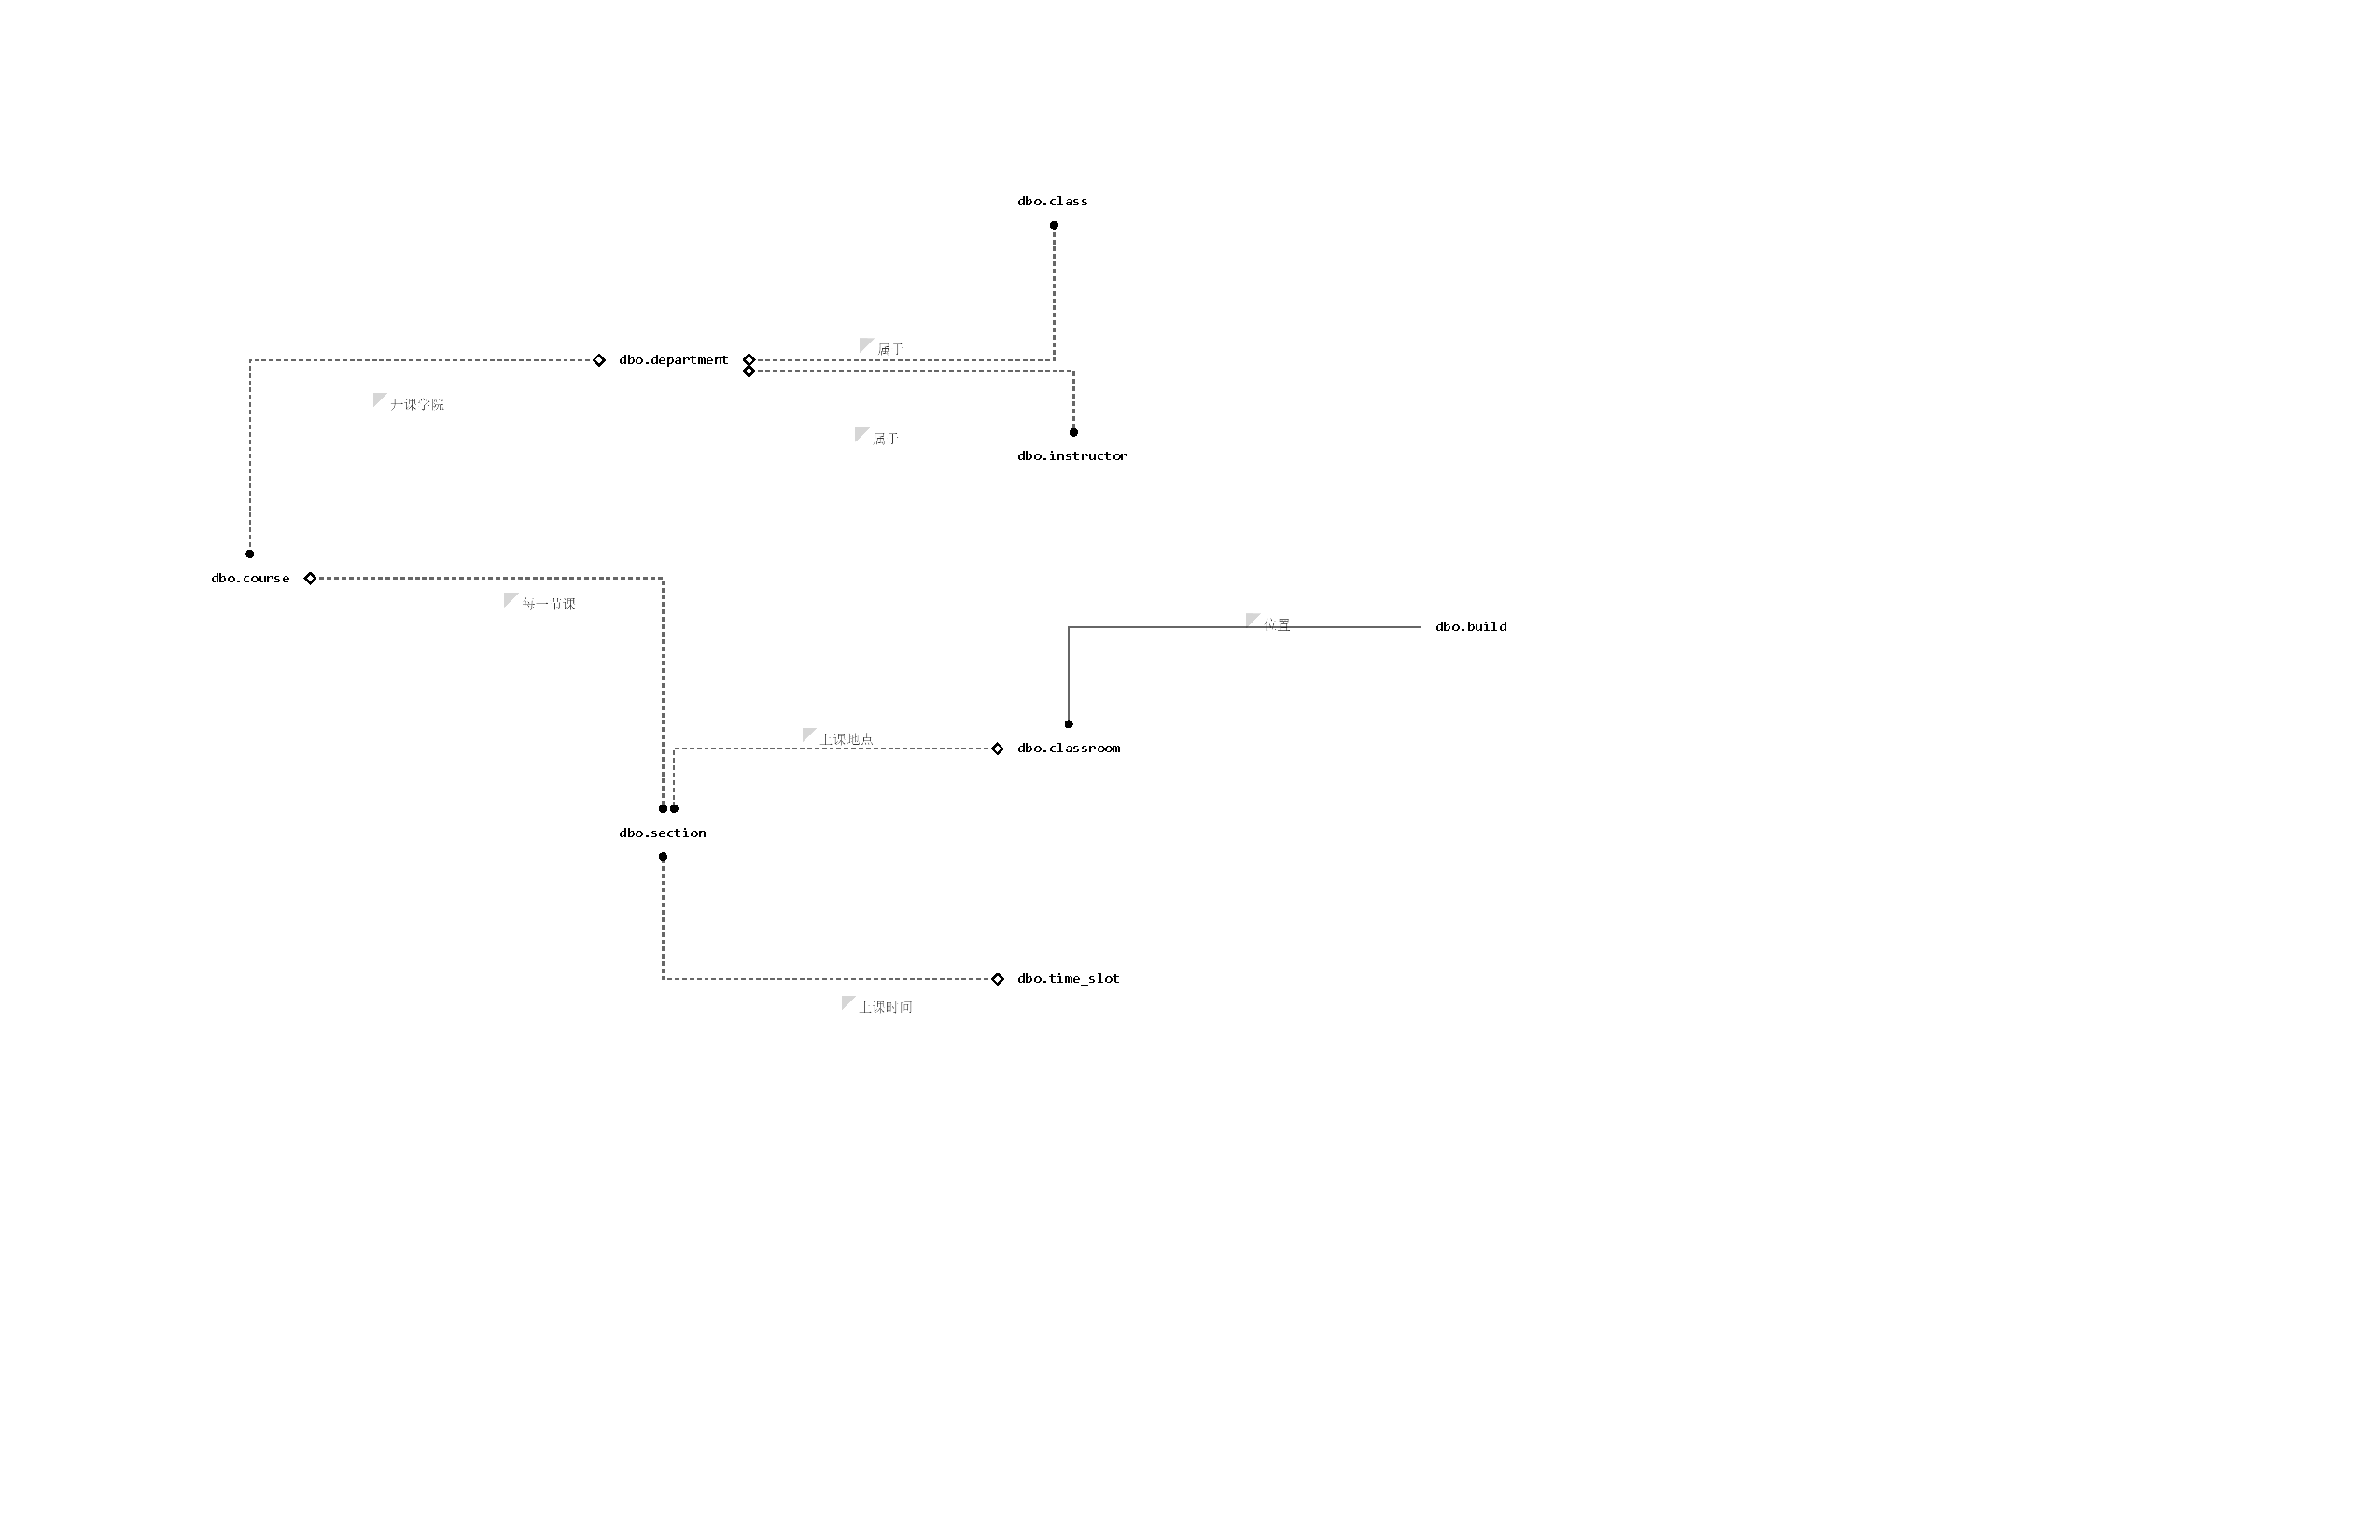
\includegraphics[width = \textwidth]{concept_model}
      \caption{数据库的概念模型(用sqlqbm制图\upcite{sqldbm})}
      \label{fig:concept_model}
    \end{figure}


\section{数据库逻辑结构设计}
  \subsection{概念模型转化为逻辑模型}
    \subsubsection{一对一关系的转化}
      % (标注主、外键)
      在数据库系统概念中\upcite{silberschatz1997database},$1:1$关系的定义为
      \begin{quote}
        An entity in $A$ is associated with \emph{at most} one entity in $B$,
        and an entity in $B$ is associated with \emph{at most} one entity in $A$.
      \end{quote}

      根据定义可以看出, 数据库里没有一一对应关系.

    \subsubsection{一对多关系的转化}
      一个 $1:n$ 联系有以下两种转换方式
      \begin{enumerate}
        \item 转换为一个独立的关系模式

          \emph{关系的属性}:与该联系相连的各实体的码以及联系本身的属性.

          \emph{关系的码}:$n$ 端实体的码.
        \item 与 $n$ 端对应的关系模式合并
          \emph{合并后关系的属性}:在 $n$ 端关系中加入 $1$ 端关系的码和联系本身的属性

          \emph{合并后关系的码}:不变
      \end{enumerate}
      与 $n$端对应的关系模式合并可以减少系统中的关系个数,一般情况下更倾向于采用这种方法.

      在本系统中, 院系对班级是$1:n$的关系,
      一个院系有多个班级, 一个班级只能属于一个院系,
      故班级表主键为\emph{班级号}, 外键为\emph{院系号},该键作为院系表的主键.
      同理课程,老师对院系也是$1:n$的关系, 为\emph{院系号}仍作为他们的外键.

      此外, \emph{教学楼}对\emph{教室}也是$1:n$关系,将\emph{教学楼号}作为教室的外键,
      教室,教学楼主键分别是他们的编号.


    \subsubsection{多对多关系的转化}
      一个 $m:n$ 联系可以转换为一个关系模式,其中:
      \begin{quote}
        \emph{关系的属性}:与该联系相连的各实体的码以及联系本身的属性

        \emph{关系的码}:各实体码的组合
      \end{quote}

      本系统中,
  \subsection{逻辑模型设计}
    % (.pdm图)
    % \cref{fig:logical_model}
    \begin{figure}[H]
      \centering
      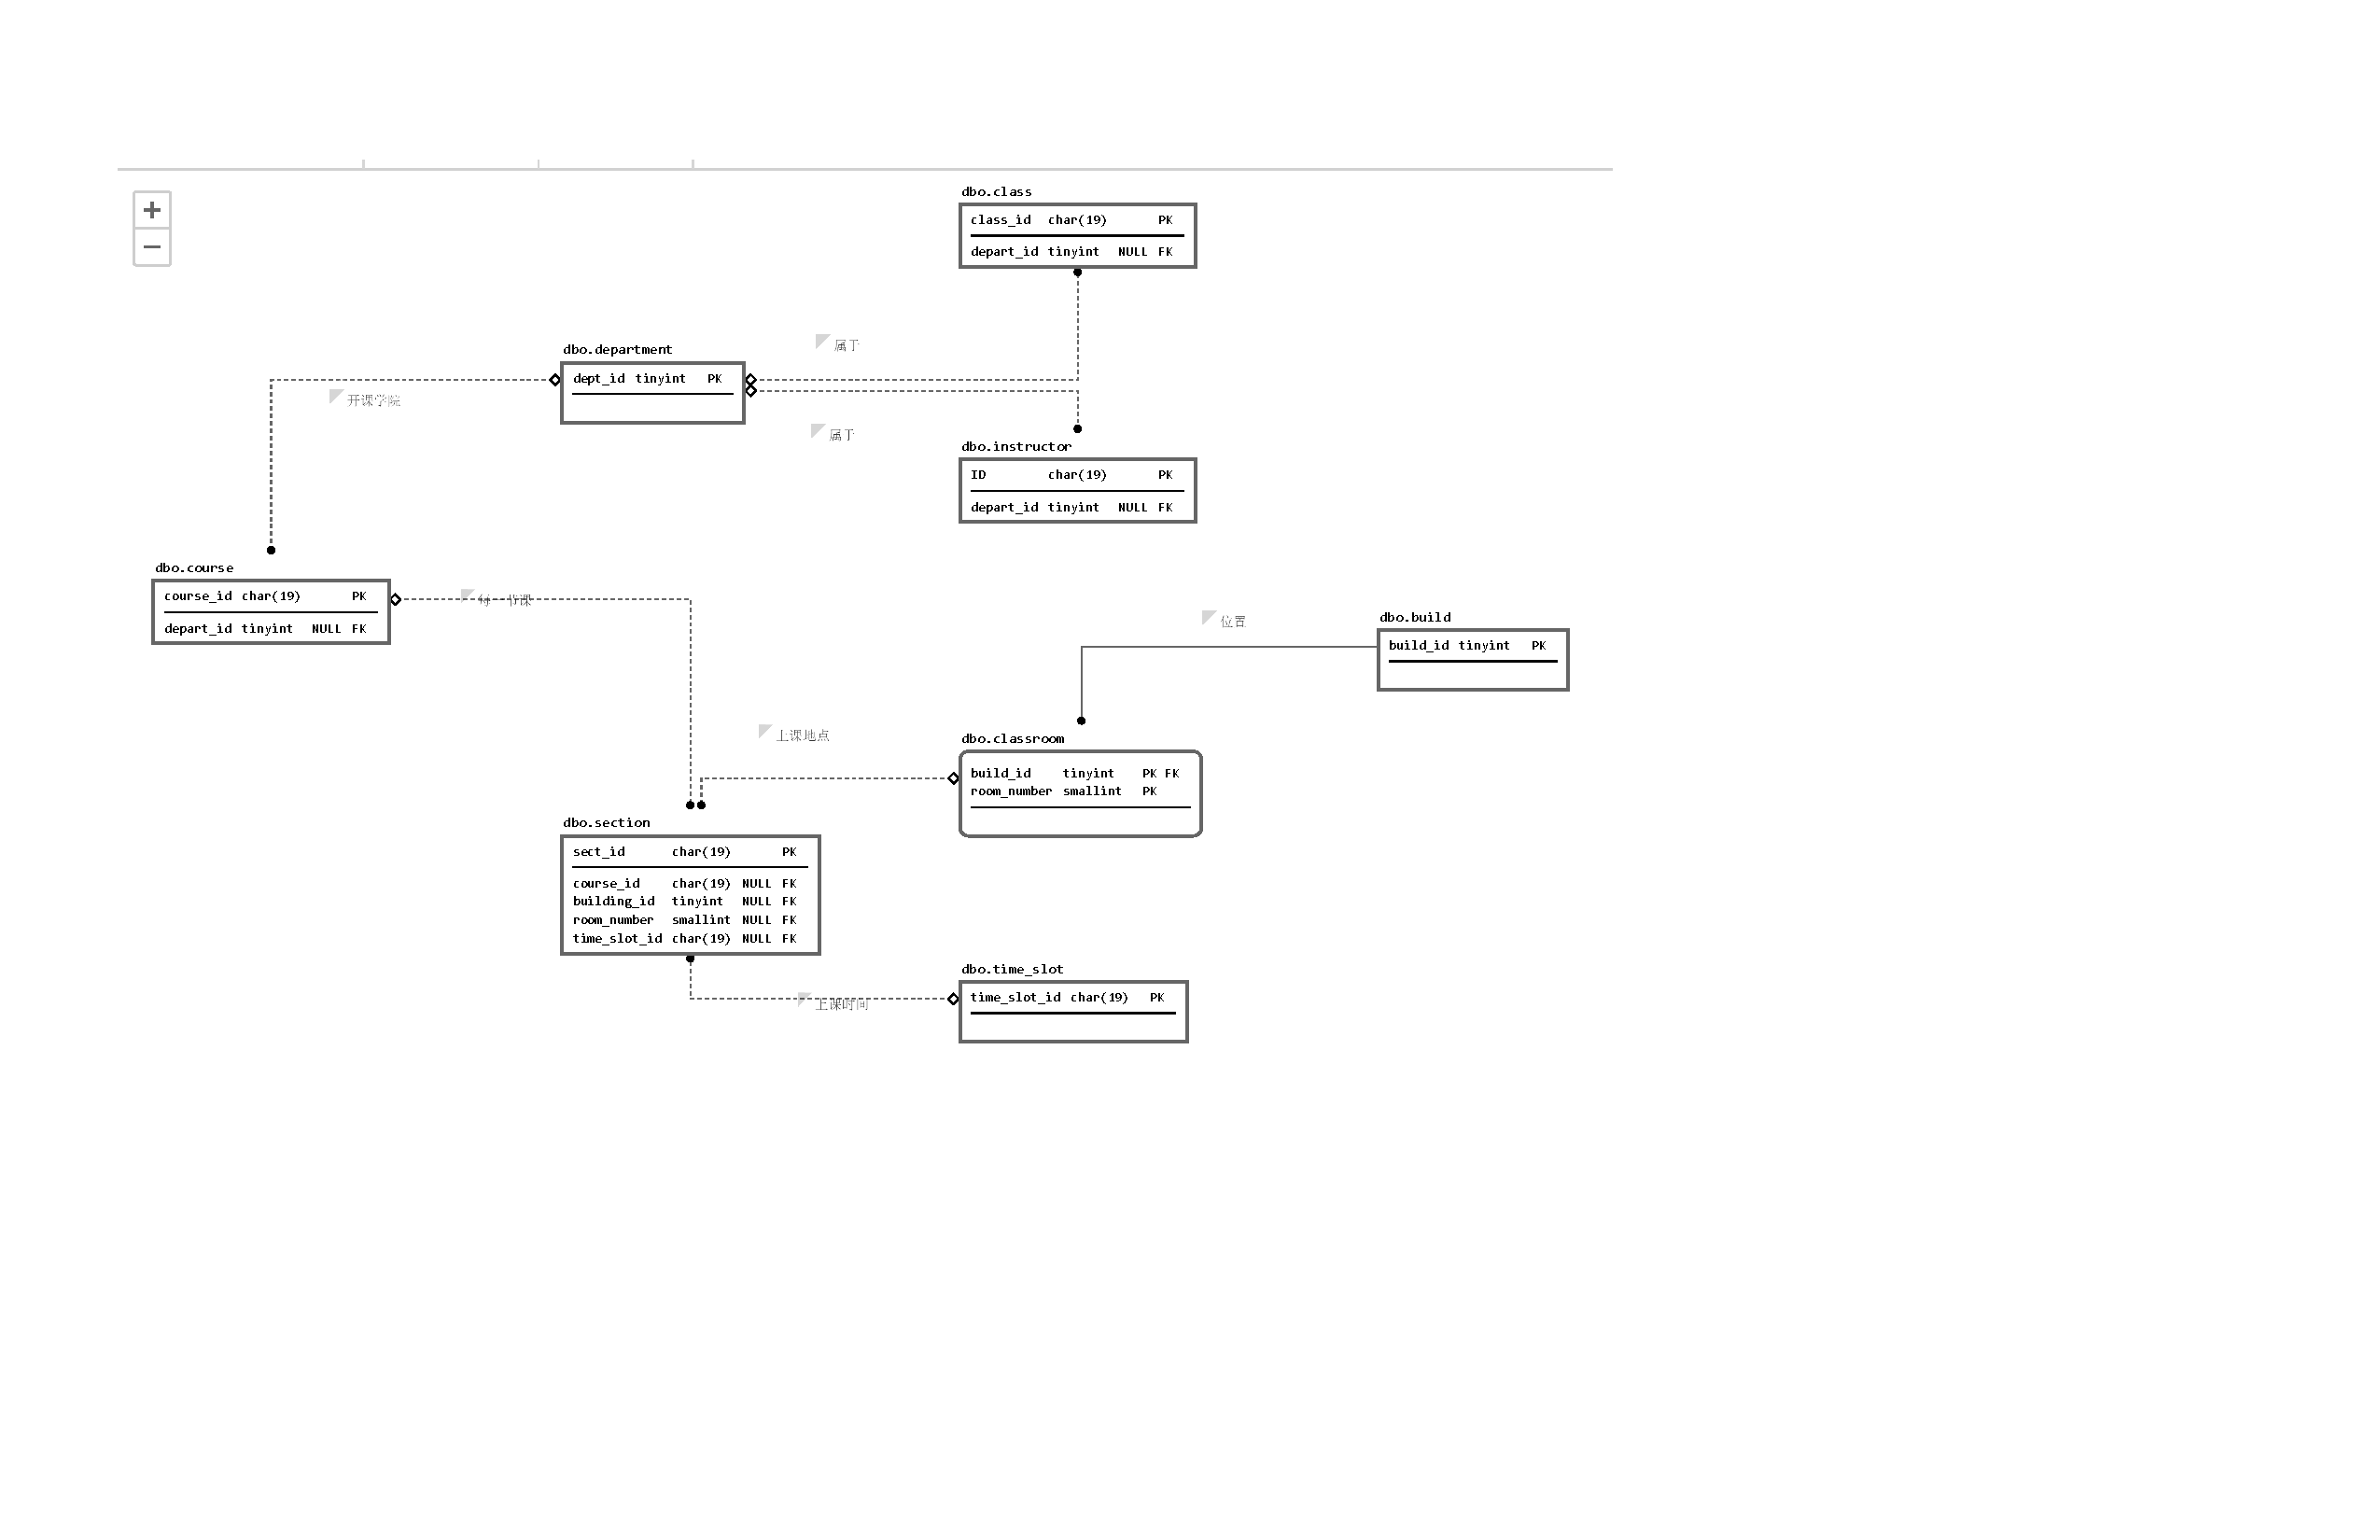
\includegraphics[width = \textwidth]{logical_model}
      \caption{逻辑结构设计}
      \label{fig:logical_model}
    \end{figure}


\section{数据库的物理实现}
  \subsection{表设计}
    % (SQL server 中各表设计)
    数据库中各表如\cref{fig:table_diagram}
    \begin{figure}[H]
      \centering
      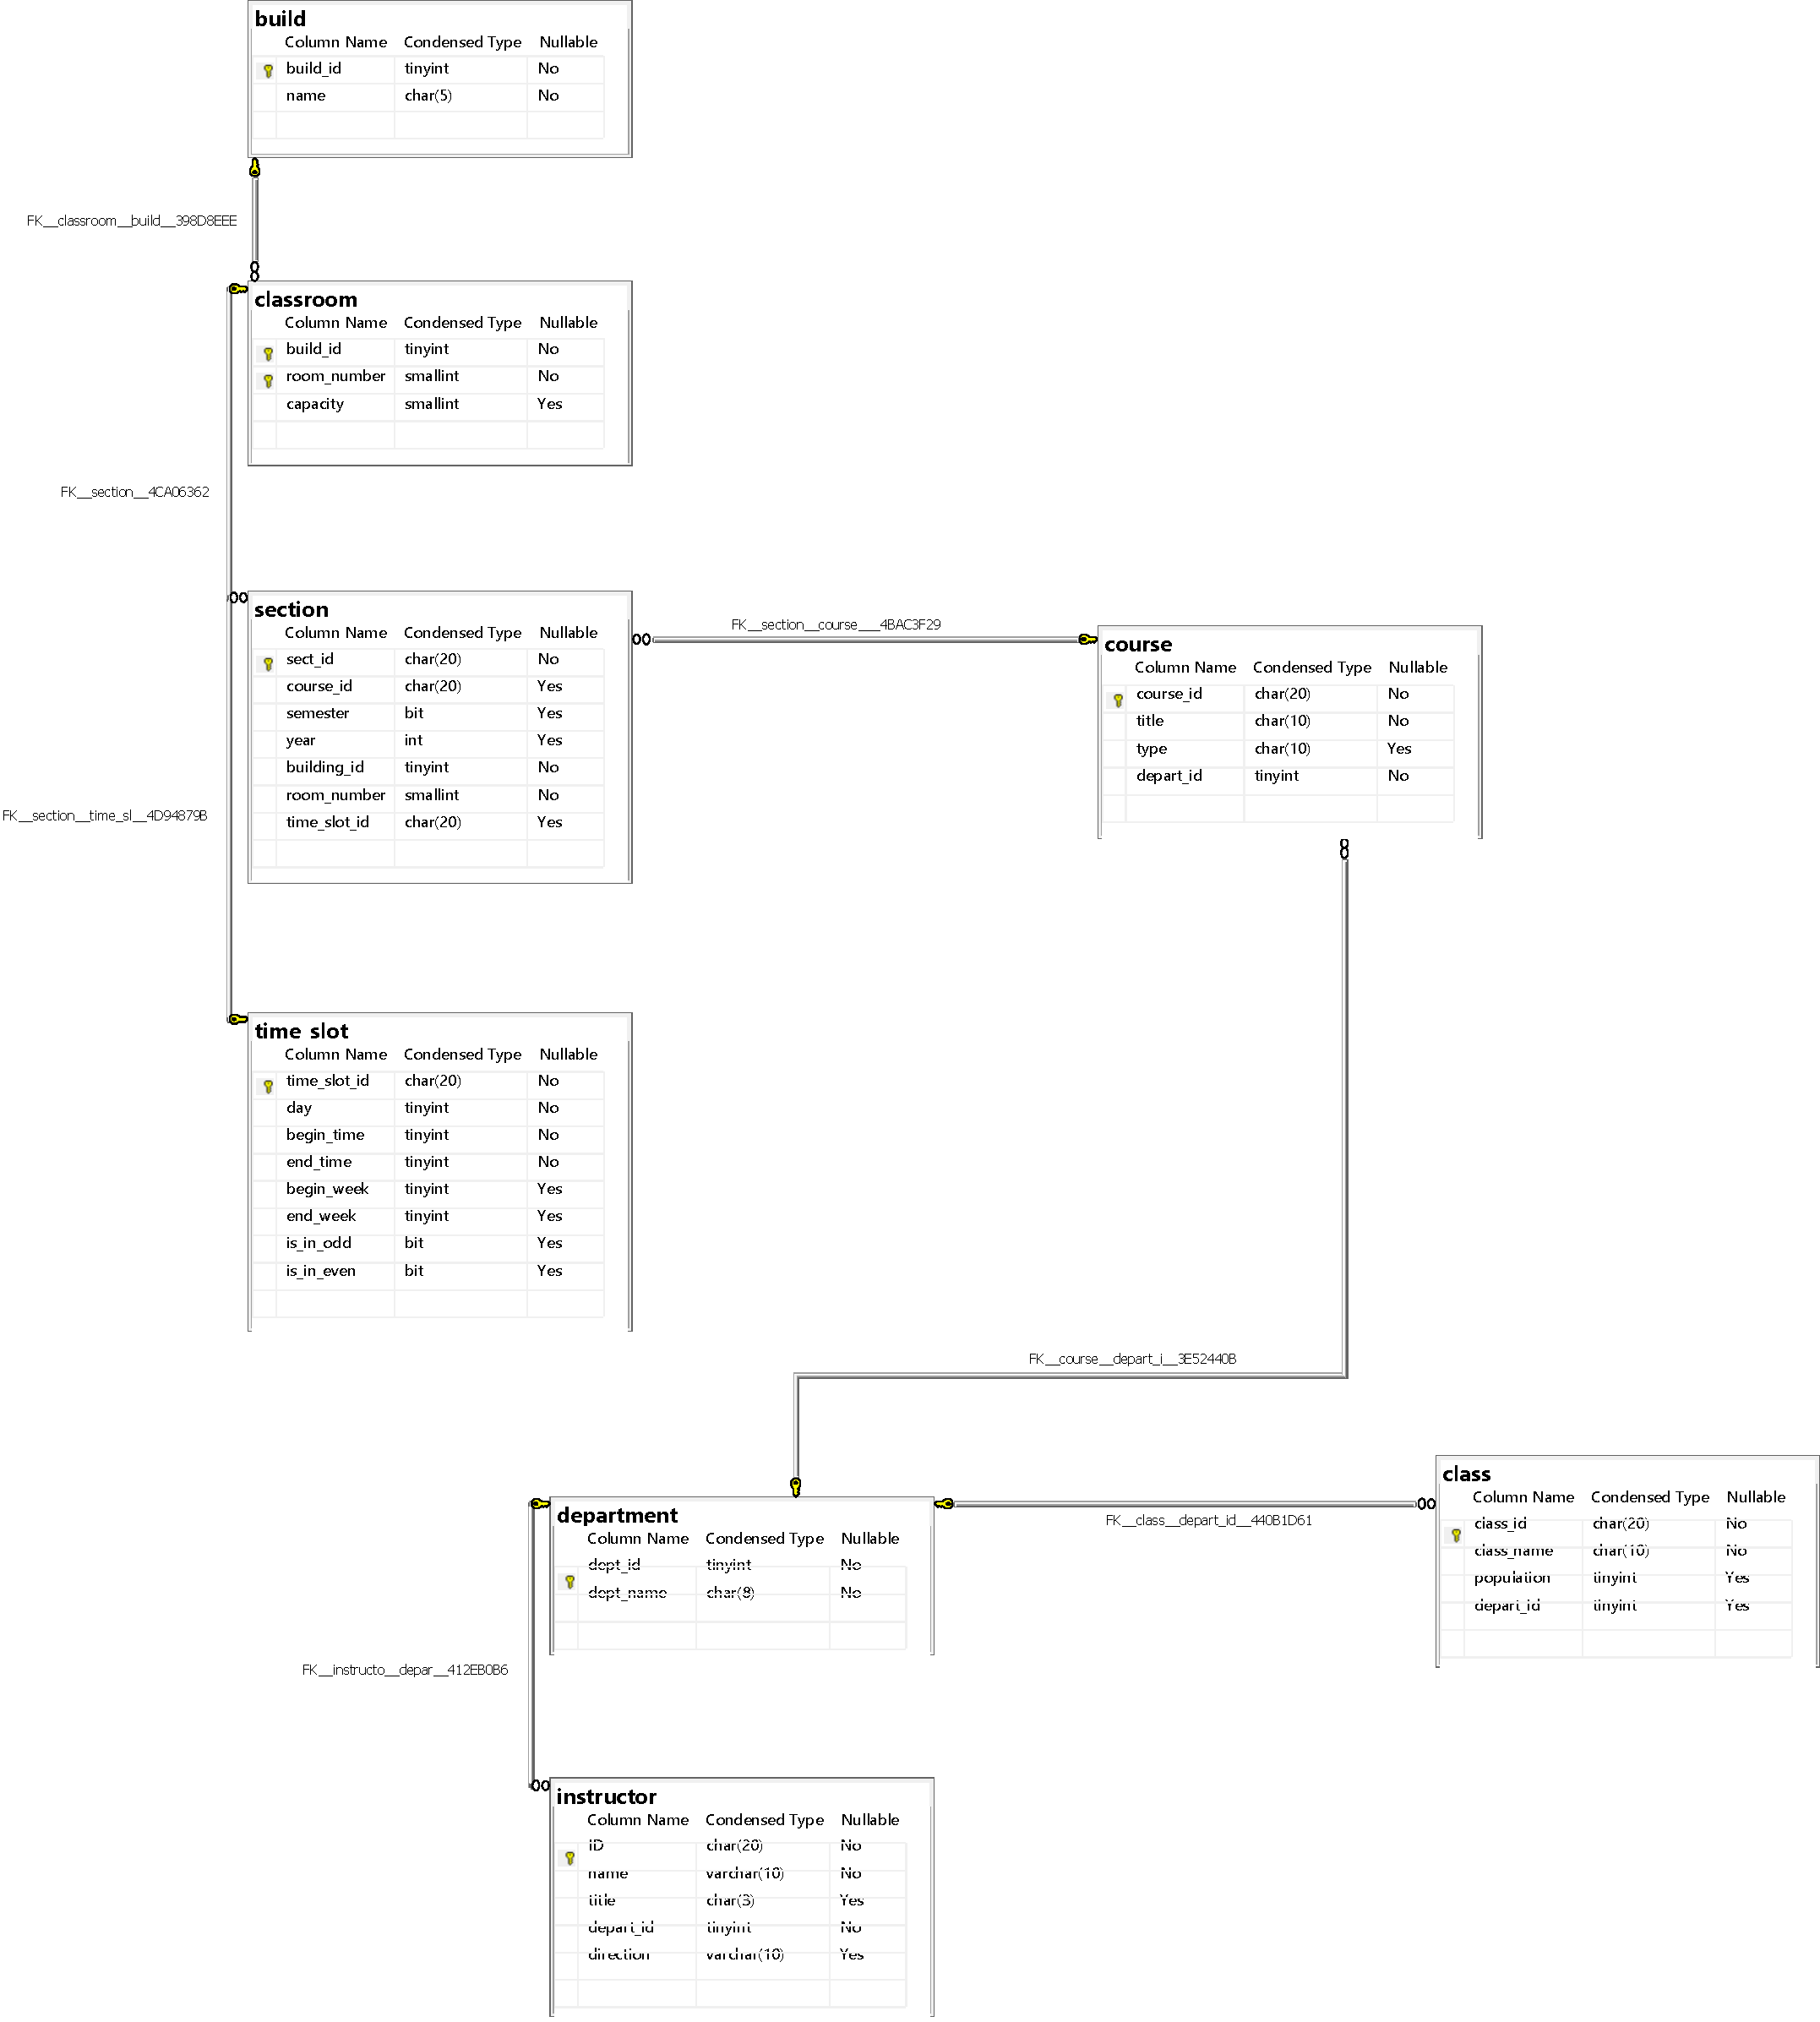
\includegraphics[width = 1\textwidth]{table_diagram}
      \caption{SQL sever 中各表设计\upcite{ssms_diagram}}
      \label{fig:table_diagram}
    \end{figure}

  \subsection{创建表和完整性约束代码设计}
    \subsubsection{\emph{教学楼}表}
    \begin{lstlisting}[language=sql]
      create table build(
        build_id tinyint,
        name char(5) not null,
        primary key (build_id),
      );
    \end{lstlisting}

    \subsubsection{\emph{教室}表}
    \begin{lstlisting}[language=sql]
      create table classroom(
        build_id tinyint,
        room_number smallint not null,
        capacity smallint,
        primary key (build_id, room_number),
        foreign key (build_id) references build,
      );
    \end{lstlisting}

    \subsubsection{\emph{院系}表}
    \begin{lstlisting}[language=sql]
      create table department(
        dept_id tinyint,
        dept_name char(8) not null,
        primary key (dept_id),
      );
    \end{lstlisting}

    \subsubsection{\emph{课程}表}
    \begin{lstlisting}[language=sql]
      create table course(
        course_id char(20),
        title char(10) not null,
        type char(10),
        instructor_id char(20) not null,

        primary key (course_id),
        foreign key (instructor_id) references instructor(ID),
      );
    \end{lstlisting}

    \subsubsection{\emph{教师}表}
    \begin{lstlisting}[language=sql]
      create table instructor(
        ID char(20),
        name varchar(10) not null,
        title char(3), /* 职称*/
        depart_id tinyint not null,
        direction varchar(10), /* 研究所或者所属系 */

        primary key (ID),
        foreign key (depart_id) references department,
      );
    \end{lstlisting}

    \subsubsection{\emph{班级}表}
    \begin{lstlisting}[language=sql]
      create table class(
        class_id char(20),
        class_name char(10) not null,
        population tinyint,
        depart_id tinyint,

        primary key (class_id),
        foreign key (depart_id) references department,
      );
    \end{lstlisting}

    \subsubsection{\emph{时间}表}
    \begin{lstlisting}[language=sql]
      create table time_slot(
        time_slot_id char(20),
        day tinyint not null,
        begin_time tinyint not null,
        end_time tinyint not null,
        begin_week tinyint default 1,
        end_week tinyint,

        is_in_odd bit default 1, /* 单周是否上课 */
        is_in_even bit default 1, /* 双周是否上课 */

        primary key (time_slot_id),
      );
    \end{lstlisting}

    \subsubsection{\emph{上课}表}
    \begin{lstlisting}[language=sql]
      create table section(
        sect_id char(20),
        course_id char(20),
        semester bit, /* 上半年或下半年 */
        year int, /* 开课年份 */
        building_id tinyint not null,
        room_number smallint not null,
        time_slot_id char(19),

        primary key (sect_id),
        foreign key (course_id) references course,
        foreign key (building_id,room_number) references classroom,
        foreign key (time_slot_id) references time_slot,
      );

    \end{lstlisting}

  \subsection{创建视图、索引、存储过程和触发器}


\section{数据库功能调试}
(包括视图、索引等内容的测试)

\section{应用程序设计}
  \begin{itemize}
    \item 项目地址:
    \url{https://github.com/chenboshuo/learn_database/tree/final_project/final_project}
  \end{itemize}
  本项目利用python的框架PyQt5 \upcite{pyqt5} 实现用户界面.

  \subsection{登录界面}
    根据\cite{pyqt5_login}的教程, 制作登录界面如
    \cref{fig:login}

    \begin{figure}[H]
      \centering
      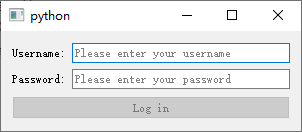
\includegraphics[width = 0.6\textwidth]{login}
      \caption{登录界面}
      \label{fig:login}
    \end{figure}
    先用模拟的账号尝试登录如
    \cref{fig:login_test}
    \begin{figure}[H]
      \centering
      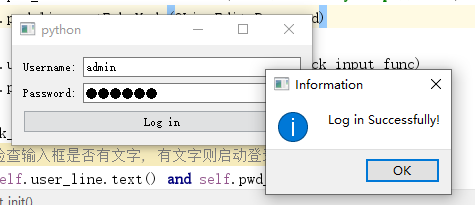
\includegraphics[width = 0.6\textwidth]{login_test}
      \caption{直接设定登录名与密码模拟登录}
      \label{fig:login_test}
    \end{figure}
    登录成功.
  \subsection{链接数据库}
    根据 \cite{connect_database} 提供的教程, 先用sql语句创建测试用户:
    \begin{lstlisting}[language=sql]
      use mytimetable;

      -- 创建一个登录账号TestUser
      create login testuser with password = '123456';

      -- 3.创建对应于这个登录账号的数据库用户TestUser
      create user testuser from login testuser ;
    \end{lstlisting}
    然后用\emph{QtSql}模块, 进行链接测试.
    % \cref{fig:test_connect}
    \begin{figure}[H]
      \centering
      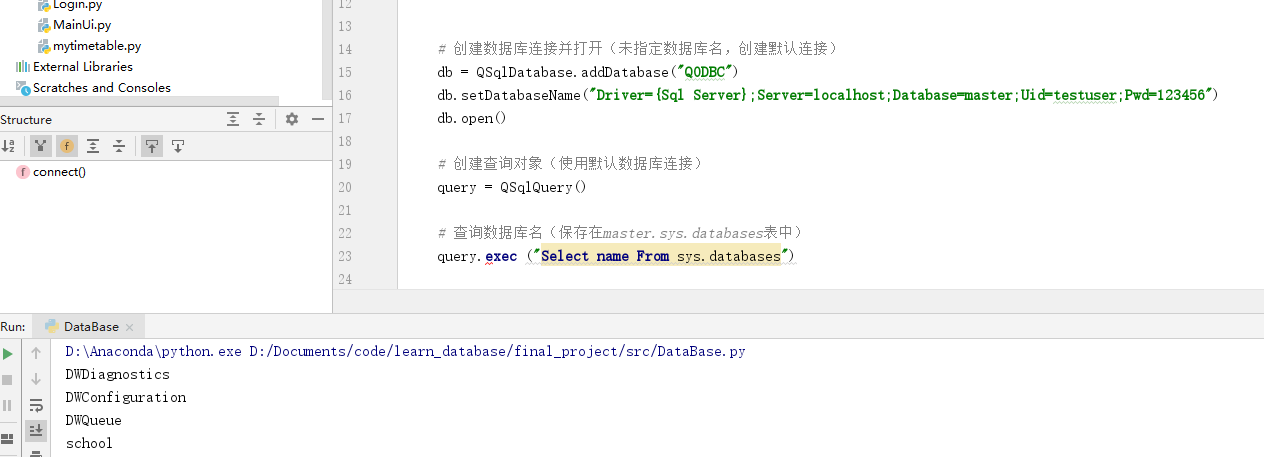
\includegraphics[width = 0.6\textwidth]{test_connect}
      \caption{测试PyQt5与sqlserver的链接}
      \label{fig:test_connect}
    \end{figure}

    测试通过后, 将该功能封装成函数,链接为数据库对象的构造函数,
    关闭为数据库析构函数,如
    \cref{fig:datebase_class_del}
    \begin{figure}[H]
      \centering
      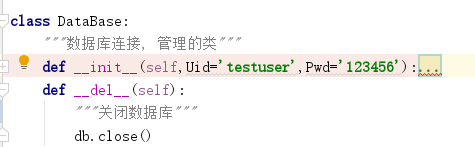
\includegraphics[width = 0.6\textwidth]{datebase_class_del}
      \caption{简单的数据库对象图}
      \label{fig:datebase_class_del}
    \end{figure}

    接下来让数据库连接:
    传递输入的变量, 尝试链接数据库,
    失败时抛出异常\upcite{pyerror}, 登录窗口检测异常,要求重新输入(\cref{fig:connect_database_error}); 若无异常, 链接(如\cref{fig:connect_database})

    \begin{figure}[H]
      \centering
      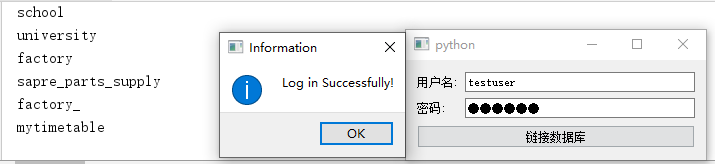
\includegraphics[width = 0.6\textwidth]{connect_database}
      \caption{连接成功后控制台打印相关信息}
      \label{fig:connect_database}
    \end{figure}

    \begin{figure}[H]
      \centering
      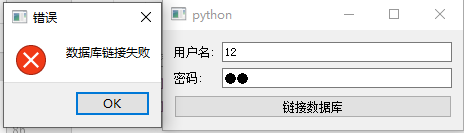
\includegraphics[width = 0.6\textwidth]{connect_database_error}
      \caption{链接失败提示并重新输入}
      \label{fig:connect_database_error}
    \end{figure}

  \subsection{主界面}
    根据 \cite{pyqt5_beautify} 提供的教程和\cite{icon}提供相关的图标样式,设计主界面如
    \cref{fig:main_ui}
    \begin{figure}[H]
      \centering
      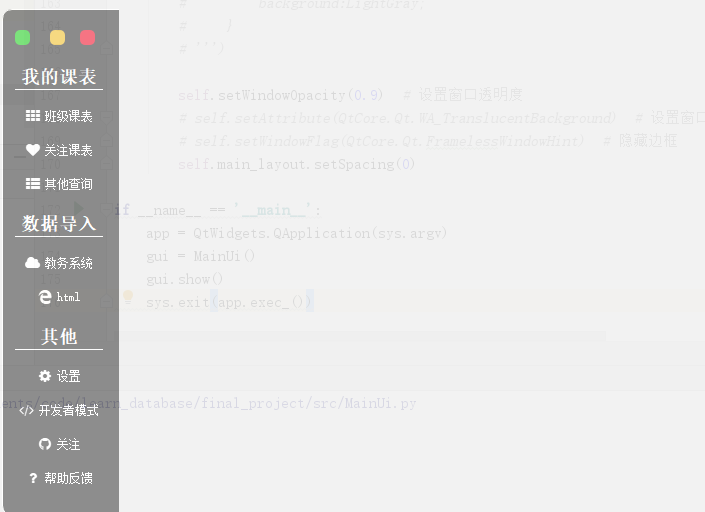
\includegraphics[width = 0.6\textwidth]{main_ui}
      \caption{程序主要功能界面}
      \label{fig:main_ui}
    \end{figure}

\section{设计总结}
  \subsection{应用改进}
    在开始设计数据库时, 是想把它当作查询课表工具使用,
    因为用教务系统查询其他学院课表时会消耗大量时间,
    这样的重复工作理应当用程序实现,
    但是查询别人课表是个小众需求, 市场上并没有课程表软件实现查询非自己班级课表的功能,所以我一直想找机会实现.

    由于课程设计要求, 需要设计多角色多过程,
    但是, 最终我希望它不是一个用于当作作业提交的系统,
    而是一个好的辅助工具, 因此在界面设计是留下一些未完成的功能,比如html转化, 在今后有时间可以将html的图表格式通过识别信息储存到数据库中实现查询,还有爬虫, 可以直接登录教务系统查询结果并保存到本地, 当然这需要大量时间.
  \subsection{其他感想}

    老师要求使用的\emph{powerdesiner}是不太好用的软件,
    现在有在线服务可以将代码转换为示意图\upcite{sqldbm},
    设计精确到代码也许能保证后面的工作可以正确进行,
    且代码的操作比用鼠标操作更高效.
    对于其他类型的图片,\url{draw.io}提供了更美观更自由,更多样的图片,并且可以自由导出\upcite{drawio},
    互联网上有大量的优质软件和服务,
    作为设计者, 不应该固步自封, 拘泥于某个软件,
    有的软件自然好用方便, 但是可能有他不擅长的功能,
    选择的时候要目光长远, 不能说能完成,
    而是更高效优雅的完成.
    比如用鼠标画图生成代码恐怕不是好主意,
    诚然, 图片的转化是逻辑转化的过程,
    但是图片一旦出错, 难以调整修改,
    绘图操作又浪费了大量时间.
    迷恋于可视化操作,当真正需要用程序调用的时候,
    又不能很好的完成,
    因为没有代码的思维甚至抵触代码,
    对我们来说可能是致命的.


    对于应用程序, 我选用了面向对象的设计思维,使用\emph{python}
    的\emph{PyQt5}可以较快的完成特别美观的界面,
    开发代码也简洁优雅, 并且有强大的界面美化库\upcite{icon},
    程序可扩充性较强,
    并且有简单的测试框架\upcite{pytest_doc}
    可以用\emph{python}的强大生态做成实用的工具.



% 参考文献
 % 数据库系统概论

\bibliography{reference} % 提示从reference数据库获取文献信息,来打印参考文献


\end{document}
